\documentclass[spanish]{fpunathesis}

\usepackage{babel}
\usepackage[utf8]{inputenc}
\usepackage[T1]{fontenc}
\usepackage{textcomp}
\usepackage[inline,shortlabels]{enumitem}
\usepackage{amsmath}
\usepackage{color}
\usepackage{booktabs}
\usepackage{cleveref}
\usepackage[section]{placeins}


\captionsetup[lstlisting]{format=mylst,labelfont=bf,singlelinecheck=off,labelsep=space}

% Cambia el nombre de "cuadro" a "tabla" cuando se usa \cref{tab:alguna_tabla}
\crefname{table}{tabla}{tablas}
\crefname{listing}{consulta}{consultas}

\graphicspath{
{capitulos/2/figuras/}
{capitulos/4/figuras/}
{capitulos/6/figuras/}
}

\begin{document}

\title{Aproximación colaborativa del tránsito vehicular basado en aplicaciones móviles}
\author{Alfredo Daniel Campuzano Romero \and Rubén Darío López Rojas}
\degree{Informática}
\advisor{Ing.}{Joaquín Quinto Lima Molinari}
\logosource{logo.png}
\maketitle

\tableofcontents
\listoffigures
\listoftables
\listofalgorithms
\lstlistoflistings

\mainmatter
\chapter{Introducción}

\section{Motivación}

La congestión de tránsito es uno de los problemas más serios que enfrentan las zonas urbanas del mundo hoy en día, tanto en países desarrollados como en países en vías de desarrollo, el constante aumento del parque de automóviles, el alto uso de vehículos de transporte privado y la falta de planificación de las ciudades son factores que deterioran la calidad de vida de los ciudadanos.

El fuerte impacto negativo de la congestión exige un esfuerzo multidisciplinario que apunte a mejorar la situación actual mediante el diseño de políticas públicas de mejoramiento de la infraestructura, la implementación de sistemas de monitoreo y control de tránsito eficientes, la mejora del sistema de transporte público y la mejora en la educación vial de la población.

Los países menos desarrollados no cuentan con sistemas integrados de control de tránsito debido al alto costo de inversión requerido, tampoco existen servicios proveídos por empresas privadas. Esta situación dificulta la utilización eficiente de las escasas y mal planificadas vías de tránsito existentes, es por eso que se hace evidente la necesidad de recolectar y analizar información sobre el tránsito de forma barata, sencilla y que requiera una mínima inversión.

En este trabajo se propone la implementación de un sistema que permitirá monitorear las condiciones del tránsito utilizando información proveída por dispositivo móviles en tiempo real. Para ello se estudiará el estado del arte de las técnicas de recolección, análisis y distribución de información de tráfico y se seleccionarán los mecanismos de monitoreo y análisis más adecuados a las necesidades y limitaciones de nuestro medio. Dicha información quedará disponible de forma pública y podrá ser utilizada en trabajos futuros para desarrollar soluciones que ayuden a mitigar la problemática de la congestión vehicular.

\section{Objetivos}

El principal objetivo de este proyecto es construir un sistema que permita recolectar y procesar información del estado del tránsito vehicular en tiempo real a través de dispositivos móviles para ofrecer funcionalidades que ayuden al control y/o reducción de la congestión de tránsito.

Entre los objetivos específicos se puede citar:

\begin{itemize}

\item Estudiar el estado del arte de las técnicas de recolección de datos de tránsito con un enfoque particular en el área de Floating Car Data.

\item Estudiar el estado del arte en técnicas de Map Matching utilizadas para procesar la información obtenida.

\item Estudiar el estado del arte de técnicas de Distribución de la Información entre dispositivos móviles.

\item Diseñar la arquitectura para un sistema que utilice las técnicas estudiadas de modo a recolectar, analizar, distribuir y utilizar la información del estado del tránsito vehicular.

\item Implementar una aplicación móvil que se utilizará para recolectar datos de ubicación de los usuarios, distribuir la información de tránsito procesada y brindar soporte a los usuarios.

\item Implementar un sistema centralizado capaz de recibir los datos de ubicación de los usuarios para determinar el estado del tránsito vehicular.

\end{itemize}

\section{Organización}

Este trabajo está dividido en 5 capítulos. El capítulo 1 describe la motivación para realizar el trabajo, brinda una visión general de los desafíos existentes y define los objetivos que se desean alcanzar.

%TODO corregir, cambio la numeración de capítulos.

En el capítulo 2 se hace un extenso estudio del estado del arte de las técnicas de recolección, análisis y distribución de los datos necesarios para la implementación del sistema, con un especial énfasis en las técnicas de Floating Car Data para la recolección de datos y de Map Matching para el análisis de los mismos.

El capítulo 3  describe el problema y se explica detalladamente la arquitectura de la solución propuesta, las técnicas seleccionadas para la recolección y el análisis de datos y los algoritmos utilizados en casa paso del proceso.

En el capítulo 4 se presenta un análisis de las pruebas realizadas para verificar el funcionamiento del sistema y muestra los resultados obtenidos. Finalmente en el capítulo 5 se presentan las conclusiones y se proponen los posibles trabajos futuros.

\chapter{Sistemas Geográficos de Información}

Se conocen como Sistemas de Información Geográfica (SIG) a aquellos sistemas basados en computadoras diseñados para la recolección, mantenimiento, análisis y distribución de datos e información geográfica [1]. Un SIG es un sistema de hardware, software, personas, datos, organización y mecanismos institucionales para recoger, almacenar, analizar y difundir información sobre las áreas de la tierra [2].

El objetivo principal de los SIG es almacenar información precisa sobre la localización de objetos de interés, así como sus propiedades y atributos. Los SIG ayudan en en el análisis y la toma de decisiones basadas en información geográfica y son aplicables en diversas áreas de la actividad humana como la planificación para el desarrollo de zonas urbanas y rurales, la delimitación de propiedades y el cobro de  impuestos, el análisis del flujo del tráfico en ciudades, entre otros. Estos sistemas proveen funcionalidades para manipular datos espaciales, calcular distancias, áreas y adyacencias entre objetos, modificar datos geográficos, realizar análisis cuantitativos y cualitativos, visualizar mapas, gráficos y tablas, etc.

En este capítulo se explican los conceptos fundamentales que sirven de base para el desarrollo de los SIG como los sistemas de coordenadas y proyecciones, los modelos de datos utilizados para representar la información geográfica y las bases de datos en las que se guarda la información.

\section{Datums, Proyecciones, y Sistemas de Coordenadas}

La tarea fundamental de un SIG es conocer la ubicación de los objetos de interés e identificar dicha ubicación dentro de un map. En esta sección describimos los principios básicos que permiten definir esta ubicación y representarla en un mapa plano.

\subsection{Sistemas de Coordenadas}

Se denominan como coordenadas al conjunto de números que identifican de forma única a una posicion dentro de un sistema de coordenadas. Estos números son representados generalmente como pares x,y en un plano cartesiano, o como latitud y longitud en un sistema de coordenadas geográficas. Para definir el sistema de coordenadas geográficas se tienen en cuenta dos elementos principales: 1) el tamaño y la forma de la tierra y 2) un conjunto de elementos de referencia a partir de los cuales se puede determinar la ubicación de cualquier otro objeto en la superficie de la tierra.

La forma de la tierra es modelada como un elipsoide achatado hacia los polos, su semieje mayor corresponde al radio en la direccion del ecuador, y su semieje menor corresponde al radio en la direccion de los polos. El factor principal para determinar la forma y el tamaño de la tierra son los  radios y el centro del elipsoide. Los polos están definidos por el eje de rotación del elipsoide y el ecuador se define como el círculo a mitad de camino entre los dos polos, en un ángulo recto con respecto al eje polar, y que cubre la dimensión más ancha de la elipsoide (Fig. 1.1). Las ubicaciones de estos elementos son estimadas utilizando mediciones  precisas. Una vez que estas localizaciones han sido estimadas se pueden especificar las coordenadas geográficas. Esto crea un sistema de referencia mediante el cual podemos especificar la posicion de objetos en la superficie del elipsoide.

Figura 1.1. Elipsoide utilizado para modelar la superficie del planeta Tierra.

La forma del elipsoide está dada por la siguiente ecuación.

Los sistemas de coordenadas geográficas se componen de la latitud, que varía de norte a sur, y la longitud, que varía de este a oeste. Las líneas de longitud constante son denominadas meridianos, y las líneas de latitud constante son denominadas paralelos. Los paralelos son líneas paralelas entre sí en dirección este-oeste alrededor de la Tierra. Los meridianos son líneas que van de sur a norte y convergen en los polos. Por convención, el ecuador se toma como la latitud de cero grados y latitudes al sur y al norte varían en un rango de hasta 90 grados. Se toma como longitud cero al meridiano que atraviesa el Observatorio Real de Greenwich, en Inglaterra y las longitudes al este u oeste se especifican como ángulos de giro con respecto al Meridiano de Greenwich, variando de -180 grados (oeste) a 180 grados (este). Ver Figura 1.2.

Figura 1.2. Sistema de coordenadas de latitud y longitud.

\subsection{Datums geodésicos}

Con el sistema de coordenadas definido se procede a estimar las longitudes y latitudes de todas las demás ubicaciones a través de mediciones. En décadas anteriores estas estimaciones se hacían utilizando técnicas astronómicas, midiendo distancias y direcciones entre puntos. Hoy en día se utilizan técnicas modernas de posicionamiento basado en satélites. Mediante estas estimaciones se establecen un conjunto de puntos de referencia para los cuales la latitud y la longitud han sido precisamente determinadas. Todas las demás coordenadas se miden con referencia a este conjunto de puntos.

Este conjunto de puntos se conoce como datum geodésico.  Un datum geodésico consta de dos componentes principales. El primer componente es un elipsoide con un sistema de coordenadas esféricas o cartesianas de tres dimensiones y un origen. La segunda parte consiste en un conjunto de puntos y líneas cuyas coordenadas han sido medidas cuidadosamente utilizando los mejores métodos y equipos.

A lo largo de la historia diferentes estudios han determinado diversos valores para los radios y el centro del elipsoide. Debido a errores de medición, diferencias en los métodos de cálculo y a que la tierra no es un elipsoide perfecto, diferentes estimaciones alrededor del mundo tienen ligeramente diferentes orígenes, ejes de orientación y radios. Estas diferencias aunque pequeñas, generalmente resultan en estimaciones bastante diferentes para las coordenadas de una misma localización,  dependiendo del elipsoide utilizado. En la actualidad las mediciones globales y la avanzada capacidad computacional permiten estimar elipsoides aplicables de forma global. Debido a esta diferencia en las estimaciones existen datums diferentes para diferentes partes de la tierra, desarrollados en distintas épocas.

El primer datum utilizado ampliamente en Norteamérica fue el North American Datum de 1927 (NAD27), su sucesor fue el North American Datum de 1983 (NAD83), las mejores estimaciones de las localizaciones de los puntos cambiaron en hasta 200 metros entre estos dos datums (ver Fig. 1.3). El World Geodetic System de 1984 (WGS84) es un conjunto de datums globales desarrollado y utilizado principalmente por el Departamento de Defensa de los Estados Unidos y hoy en día es ampliamente aceptado y utilizado en todo el mundo.

Figura 1.3a. Desplazamiento de la latitud de los datums en metros, NAD83 menos NAD27.

Figura 1.3a. Desplazamiento de la longitud de los datums en metros, NAD83 menos NAD27.

\subsection{Proyecciones}

Una proyección es una representación sistemática de las posiciones de la superficie de la curva Tierra sobre una superficie plana de un mapa. El mapa resultante sufre una distorsión debido a la traducción de una superficie superficie curva a una superficie plana. Diferentes proyecciones pueden distorsionar el mapa de diferentes maneras. La proyección puede definirse por lo tanto como la transformación de una posicion en la superficie de la tierra, identificada por su latitud y longitud
%(f, ?),
a una posicion en coordenadas cartesianas (x, y). Cualquier proyección puede representarse como un par de funciones matemáticas:

%x = f (f,?)
%y = g(f, ?)

Las proyecciones se pueden clasificar de acuerdo a su forma, en cónicas, cilíndricas o planas (Fig. 1.4) y de acuerdo a su orientación en ecuatoriales, cuando por ejemplo el eje de un cilindro coincide con los polos, o transversales, cuando por ejemplo el eje del cilindro coincide con el ecuador.

Figura 1.4. Tipos de proyecciones: a) cilíndrica, b) cónica y c) plana.

Algunas de las proyecciones más importantes son la Proyección Cilíndrica Equidistante, que produce una imagen fuertemente distorsionada de la Tierra con los polos extendidos a lo largo de la totalidad de los bordes superior e inferior del mapa (Fig. 1.5); la Proyección Conforme de Lambert, que se obtiene interceptando un cono con la superficie de la tierra en dos paralelos del elipsoide; la Proyección Transversa de Mercator, que se obtiene envolviendo la Tierra con un cilindro y proyectando las posiciones de la misma sobre el cilindro, el eje del cilindro se encuentra en el plano ecuatorial y el Sistema de Coordenadas Universal Transversal de Mercator (UTM por sus siglas en Inglés), que está basada en la Proyección Normal de Mercator pero en lugar de ser tangente al ecuador es tangente a un meridiano, es decir es un cilindro cuyo eje es el eje polar del elipsoide.

Figura 1.5. Proyección Cilíndrica Equidistante (Plate Carrée)

\section{Modelos de datos}

Una vez que tenemos definidos el sistema de coordenadas y que podemos representar conceptualmente la localización de los objetos en un mapa, el siguiente paso es definir una estructura de datos que represente esta información de manera a que la misma pueda ser manipulada y analizada con un SIG. En esta sección describimos brevemente las estructuras de datos comúnmente utilizadas en los SIG actuales.

\subsection{Modelo de Datos Vectorial}

En un modelo vectorial cada objeto del mundo real es representado como uno de tres posibles tipos de datos geométricos: puntos, líneas o polígonos (Fig. 1.6). Un punto se representa de forma única por sus coordenadas (ciudades, puestos de salud, comisarías), las líneas se representan como una lista ordenada de coordenadas correspondientes a sus vértices (rutas, ríos y arroyos) y los polígonos se representan como uno o más segmentos de líneas que se cierran para formar un polígono (propiedades rurales, lagos, delimitación de distritos). Las coordenadas que definen la geometría de cada objeto pueden tener 2, 3, 4 o más dimensiones. En algunos modelos de datos las figuras geométricas pueden ser representadas por curvas definidas por una función matemática (ej. curvas de Biézer).

Figura 1.6. Representación vectorial.

Objetos del mismo tipo (ej. calles) normalmente son guardadas en una tabla de base de datos en la que cada objeto ocupa una fila de la tabla y cada atributo del objeto corresponde a una columna de la tabla. En un SIG también se puede almacenar información topológica sobre los objetos. La topología es la ciencia que estudia las relaciones geométricas entre las distintas figuras y objetos geométricos (puntos, líneas, polígonos), por ejemplo las relaciones de adyacencia y conectividad. Las relaciones topológicas son propiedades cualitativas de los objetos geográficos que permanecen constantes cuando se distorsiona el espacio geográfico de los objetos.  Por ejemplo para cada calle se puede definir su sentido de circulación y su límite de velocidad.

\subsection{Modelo de Datos Raster}

En una representación raster el espacio es dividido en una colección de celdas rectangulares, todas las variaciones geográficas son expresadas asignando propiedades o atributos a estas celdas. Este tipo de representación requiere que la superficie curva de la tierra sea proyectada en una superficie plana. Debido a que esto genera distorsiones, las celdas en una representación raster no son perfectamente iguales en forma o área a la superficie que representan. Cuando se usa este formato, toda la información acerca de las variaciones dentro de una celda es perdida y se asigna un único valor a toda la celda (Fig. 1.7).

Figura 1.7. Representación raster.

Las celdas pueden contener atributos basado en diversos esquemas de codificación. Por ejemplo, un esquema de codificación simple puede asignar un valor binario, cero o uno, a cada celda para representar la presencia o ausencia de forestación en dicha celda. En casos más avanzados se utilizan números de punto flotante para representar por ejemplo el nivel de elevación de cada celda con respecto al nivel del mar. Múltiples atributos pueden ser guardados para cada celda en una tabla en la que cada columna es un atributo de la celda y cada fila representa a una celda en particular. Los datos usualmente son guardados en archivos comprimidos o en bases de datos relacionales.

\subsection{Modelos de Datos de Red}

El modelo de red es un tipo especial de modelo topológico que puede ser utilizado para modelar el flujo de bienes y servicios. En un SIG las redes son modeladas como puntos o nodos (ej. intersecciones de calles, fusibles, interruptores, válvulas de agua) y líneas  (calles, líneas de transmisión y tuberías).  Las relaciones topológicas de la red definen  cómo las líneas se conectan entre sí en los nodos y también pueden definir reglas sobre cómo los flujos pueden moverse a través de una red.

Por ejemplo, en una red de calles que está compuesta por un conjunto de nodos (intersecciones de las calles) y líneas (las calles), así como las relaciones topológicas entre las mismas (restricciones de giro en los nodos, sentido de las calles, límites de velocidad), la información topológica permite analizar el flujo de tráfico a través de la red y determinar los puntos más congestionados o calcular caminos más cortos de un punto de la red a otro.

\subsection{Red Irregular de Triángulos (TIN)}

Los modelos de datos geográficos descritos hasta ahora se utilizan para representar datos en una o dos dimensiones. Para representar superficies tridimensionales en un SIG se pueden utilizar modelos raster o redes irregulares de triángulos (TIN por sus siglas en Inglés). En los modelos raster cada celda almacena la altura de la superficie en una localización dada. En una estructura TIN se representa una superficie como una serie de elementos triangulares contiguos que no se superponen entre sí.

Una estructura de datos TIN es una estructura topológica que almacena información acerca de los nodos que comprenden cada triángulo y los vecinos de cada triángulo. El triángulo está representado por una secuencia de tres nodos, cada nodo está definido por sus coordenadas x, y, z (Fig. 1.8). Los triángulos tienen como atributos su pendiente, orientación y área, los vértices tienen atributos de elevación y los bordes tienen como atributos su pendiente y dirección. Al igual que en los demás modelos de datos, cada triángulo puede tener otros datos o atributos asociados.

Figura 1.8. Representación TIN.

\section{Bases de Datos Espaciales}

Una base de datos espacial es aquella en la que están definidos tipos de datos especiales para representar objetos geométricos y permite guardar estos objetos geométricos, que usualmente son de origen geográfico, en tablas regulares de una base de datos. Además provee funciones e índices para consultar y manipular estos datos [3]. Las bases de datos espaciales no necesitan ser relacionales pero muchas de las más populares lo son.

En las bases de datos espaciales típicamente se definen tipos de datos que representan puntos, líneas y polígonos a partir de los cuáles se pueden construir otros tipos de datos más complejos y representar objetos del mundo real. Estas bases de datos están especialmente diseñadas para representar información en dos dimensiones en formato vectorial, pero también pueden almacenar datos raster y topologías tridimensionales.

\subsection{Análisis espacial, procesamiento espacial, y consultas espaciales}

Una consulta espacial es una consulta de base de datos que utiliza funciones geométricas para responder preguntas acerca del espacio y de los objetos en el espacio. Extensiones para bases de datos como PostGIS y Oracle Spatial agregan un conjunto de funciones a las ya existentes en el lenguaje SQL estándar que trabajan con objetos geométricos de forma similar a como las funciones estándar trabajan con las fechas.

Por ejemplo, existen funciones que indican la cantidad de tiempo que hay entre dos fechas o si una fecha dada corresponde al pasado o al futuro. De forma similar las base de datos espaciales proveen funciones especiales que permiten obtener la distancia entre dos figuras geométricas, o el área total de un polígono. Las funciones espaciales también permiten crear y modificar objetos geométricos.

Existen estándares que definen este conjunto de tipos de datos y funciones espaciales. Open Geospatial Consortium (OGC) es un consorcio internacional de la industria cuyo objetivo es tratar de estandarizar la forma en que los datos geométricos y espaciales son accedidos y distribuidos. OGC cuenta con numerosas especificaciones que definen el acceso a los datos geoespaciales, servicios web para consulta y manipulación de datos, formatos de datos geoespaciales y consulta de datos geoespaciales.

\subsection{Productos comerciales y de código abierto}

Existen varias bases de datos espaciales disponibles en el mercado que implementan los estándares OGC, tanto de código abierto como soluciones comerciales. Entre las bases de datos de código abierto más populares podemos citar a SpatialLite/SQLite, PostgreSQL/PostGIS y MySQL. Los productos comerciales más populares incluyen a Oracle Spatial y SQL Server de Microsoft.

PostGIS es una extensión para PostgreSQL que agrega soporte para tipos de datos geométricos y funciones especiales convirtiendo a PostgreSQL en una base de datos espacial. PostGIS es un proyecto de código abierto que se publica bajo la Licencia Pública General de GNU. Además de los tipos de datos básicos provee otros tipos de datos más complejos como multi-polígonos, multi-puntos, multi-líneas y curvas geométricas. PostGIS 2 además agrega soporte para datos raster para  y datos tridimensionales en formato TIN así como también funciones para trabajar para comparación de objetos tridimensionales. De forma similar SpatialLite es una extensión para SQLite que agrega soporte para tipos de datos y funciones geométricas.

Oracle Spatial es una extensión para la base de datos Oracle que proporciona tipos de datos y funciones para la gestión de datos espaciales. Los tipos estándar y funciones de Oracle (CHAR, DATE, INTEGER, etc) se extienden con equivalentes geográficos. Oracle Spatial provee tipos básicos de geométricas: puntos, líneas y polígonos (incluyendo polígonos complejos con agujeros), a partir de los cuáles se pueden construir estructuras de datos más complejas. Además, Oracle Spatial puede almacenar y administrar datos de tipo raster.

\chapter{Recolección de datos de tráfico}
\label{cap:3}

Actualmente existen una variedad de tecnologías para la recolección automática de datos del tráfico. Según Mimbela \cite{mimbela2003summary} podemos dividir estas tecnologías en dos. La primera es la \emph{tecnología in-situ}, que toma los datos del tráfico a través de detectores ubicados a lo largo del camino y que vuelve a dividirse en dos categorías: la intrusiva y la no intrusiva. La segunda, denominada \emph{Floating Car Data} (FCD), es una alternativa para obtener datos del tráfico de gran calidad mediante el uso de vehículos sonda equipados con dispositivos de medición que pueden ser dedicados o no.

\section{Tecnologías in-situ}

Las \emph{tecnologías de detección in-situ} se basan en la recolección de datos mediante dispositivos específicos para este fin que son dispuestos físicamente en los lugares sujetos de medición. Se dividen en dos categorías: \begin{enumerate*}[a)] \item las tecnologías \emph{intrusivas}, que están montadas en o por debajo de la superficie de las rutas y cuya instalación ocasiona la interrupción potencial del tráfico y \item las tecnologías \emph{no intrusivas}, que son montadas encima o sobre la superficie de las rutas y su instalación no genera interrupción del tráfico o lo hace en pequeña medida.\end{enumerate*}

\subsection{Sensores de tecnología intrusiva}

Los tipos de sensores y la ubicación de los mismos se pueden observar en la \Cref{fig:intrusiva}. El primer tipo de unidades son los \emph{sensores magnéticos pasivos} o  \emph{magnetómetros} que pueden ser montados de forma permanente en hoyos a lo largo del camino, o pegados a la superficie de la ruta. Estas unidades se comunican a una estación de procesamiento cercana utilizando cables debajo del camino o a través de comunicación inalámbrica. El sensor tiene una zona circular o elíptica de alcance de detección. Los magnetómetros monitorean la fluctuación en la fuerza del campo magnético, el cual cambia en presencia de objetos de metal moviéndose a través del mismo.

\begin{figure}[h]
	\centering
	\includegraphics[width=0.7\textwidth]{capitulos/3/figuras/figura1.jpg}
	\caption{\label{fig:intrusiva} Típicas configuraciones de detección intrusiva}	
	%TODO cambiar el texto 3 del gráfico por Detectortes de inducción %
\end{figure}

Un segundo tipo de unidades utiliza \emph{tubos neumáticos} que son extendidos a través de la calzada y que se fijan en la acera en ambos extremos. Una ráfaga de presión de aire se produce en el tubo de goma cuando un vehículo pasa por encima. El pulso de presión de aire cierra un interruptor produciendo una señal eléctrica que es transmitida.

El tercer tipo son los \emph{detectores de bucle de inducción}, que consisten en rollos de alambre recubierto, enterrados en ranuras cortadas en la superficie de la carretera y sellados con masilla. Los datos son enviados a través de un cable enterrado con los bucles hasta una unidad de procesamiento. Una señal eléctrica es aplicada al bucle, la cual oscila en presencia de un vehículo en movimiento. Estos cambios son detectados por la unidad de procesamiento que genera un evento que es transmitido.

Otro tipo de detector intrusivo, denominado \emph{weigh-in-motion} mostrado en la \Cref{fig:Weight-In-Motion}, consisten en un sensor piezoeléctrico ubicado en un canal a través del camino. El sistema registra la variación de tensión medida en los piezoeléctricos, lo cual genera un evento que es transmitido para su procesamiento. Estos sistemas  se utilizan en ubicaciones específicas mayormente para el control de acceso.

\begin{figure}[h]
	\centering
	\includegraphics[width=0.7\textwidth]{capitulos/3/figuras/figura2.jpg}
	\caption{\label{fig:Weight-In-Motion}  Sistema de detección weight-in-motion}	
\end{figure}

\subsection{Sensores de tecnología no intrusiva}

Los sensores de tecnología no intrusiva incluyen:  recolección de datos por video, detectores infrarrojos pasivos o activos, radares de microondas, detectores ultrasónicos, detectores acústicos, detectores láser y fotografía aérea. La mayoría de los sistemas no intrusivos son operacional y visualmente similares, consistiendo en pequeñas unidades electrónicas montadas en contenedores a prueba de agua.

\begin{figure}[h]
	\centering
	\includegraphics[width=0.7\textwidth]{capitulos/3/figuras/figura3.jpg}
	\caption{\label{fig:noIntrusica}  Configuraciones típicas de tecnologías no intrusivas}	
\end{figure}

En la \Cref{fig:noIntrusica} pueden notarse una disposición de 3 tipos de deterctores no intrusivos. El primer tipo corresponde a los \emph{montados en mástil} al costado de la carretera, tales como cámaras fotográficas o de video, capaces de procesar un campo de visión que cubre un área oblicua, ya sea por encima o por debajo de la unidad.  Problemas de oscurecimiento pueden ocurrir cuando vehículos grandes cubren a vehículos pequeños del detector o cuando el campo de visión es muy grande, causando la detección de vehículos fuera del carril deseado.

El segundo tipo de detectores no son los \emph{montados debajo de puentes o portales}, con un campo de visión justo por debajo de los mismos, o ligeramente oblicuo a la unidad. Este tipo de detectores también está sujeto a los problemas de oscurecimiento mencionados anteriormente.

Finalmente, el tercer tipo, conocidos como de \emph{fuego cruzado}, consiste en unidades tales como monitores de polución que son montados a nivel del piso a ambos lados del camino, disparando un haz a través de la carretera. Estas unidades están sujetas al enmascaramiento de lado a lado, por lo tanto, son más adecuadas para un solo carril.

\section{Tecnologías de Floating Car Data}

Además de la utilización de tecnologías in-situ, muchas aplicaciones de gestión de tráfico utilizan dispositivos montados en vehículos en circulación, conocidos como sistemas de ubicación automática de vehículo (\emph{Automatic Vehicle Location} - AVL). Los dispositivos AVL pueden proveer dos tipos de información: \begin{enumerate*}[a)]
\item información de posición, cuando un vehículo equipado con ellos pasa cierto punto de la red donde existe un sensor, o \item información continua, a medida que el vehículo transita a través de la red.
\end{enumerate*}

Los primeros sistemas AVL se basaron en vehículos equipados con transpondedores que transmitían y recibían información de los dispositivos ubicados en la carretera. Los sistemas actuales se basan en la tecnología del Sistema de Posicionamiento Global (\emph{Global Positioning Systen} - GPS) o en otros mecanismos de posicionamiento para luego transmitir la posición del vehículo.

El principio de FCD es recolectar datos de tráfico en tiempo real ubicando los vehículos a través de dispositivos AVL en toda la red de caminos como se muestra en la \Cref{fig:ComunicacionGPS}. Todos los vehículos equipados con estos dispositivos actúan como sensores dentro de la red de caminos. Datos como la ubicación del vehículo, la velocidad y dirección del viaje son enviados a un centro de procesamiento para la recolección y extracción de información. Luego de la recolección y extracción, información útil como el estado del tráfico y rutas alternativas pueden ser derivadas y posteriormente distribuidas.

\begin{figure}[h]
	\centering
	\includegraphics[width=0.7\textwidth]{capitulos/3/figuras/figura4.jpg}
	\caption{\label{fig:ComunicacionGPS}  Comunicación con GPS}	
\end{figure}

\subsection{FCD basado en GPS}

% Actualmente existen dispositivo AVL que cuentan con sensores GPS. 

Hoy en día la tecnología GPS se encuentra altamente disponible, lo que se refleja en el aumento del número de vehículos y dispositivos móviles equipados con este sistema de ubicación. Esto lleva al desarrollo de trabajos que aprovechan esta tecnología para la obtención de FCD \cite{giovannini2011novel,li2007practical,sevlian2010travel,yin2004weight}

% Esta tecnología permite obtener la ubicación con una precisión relativamente alta, típicamente menor a 30 metros. Generalmente, los datos del tráfico que se obtienen de vehículos privados o camiones con tecnología GPS son más adecuados para autopistas y zonas rurales.

A pesar de la existencia de sistemas FCD que utilizan vehículos sonda equipados con dispositivos AVL basados en GPS \cite{simmons2002commercial,leduc2008road}, que son utilizados como fuente de información en tiempo real. Su aplicación está restringida a un limitado número de vehículos debido a los costos del equipamiento dedicado requerido. 

En comparación, estrategias FCD basadas en dispositivos no dedicados, tales como teléfonos celulares u otros dispositivos móviles, que evitan los costos de equipamiento, son una alternativa que actualmente está recibiendo especial atención \cite{thiagarajan2010cooperative,thiagarajan2009vtrack,de2008traffic}.

\subsection{FCD basado en dispositivos móviles}

La rápida expansión de los teléfonos y dispositivos inteligentes y los múltiples sensores que poseen los mismos, los convierte en una potencial fuente para implementación de sistemas FCD. Muchos trabajos se centran en la utilización de dispositivos móviles para la detección del tráfico, la mayoría aprovechando los sistemas A-GPS\footnote{http://es.wikipedia.org/wiki/GPS\_Asistido}, pero también existen otros que utilizan las redes GSM\footnote{http://en.wikipedia.org/wiki/GSM}, WiFi\footnote{http://en.wikipedia.org/wiki/Wi-Fi} y hasta la tecnología Bluetooth\footnote{http://en.wikipedia.org/wiki/Bluetooth} \cite{thiagarajan2010cooperative,thiagarajan2009vtrack,fraser2007use,fang2011enacq,ruppe2012augmenting}.

En 2007, Fraser \cite{fraser2007use} habla de la viabilidad de utilización de dispositivos móviles como alternativa a los métodos típicos de detección de tráfico, utilizando ubicación de objetos mediante triangulación con antenas de telefonía, tal como se muestra en la \Cref{fig:triangulacionAntenas}. En el mismo trabajo se comenta de las dificultades que tienen tales sistemas en cuanto a la precisión de ubicación, quedando este punto como una problemática a ser resuelta.

\begin{figure}[h]
	\centering
	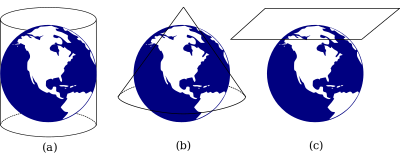
\includegraphics[width=0.7\textwidth]{capitulos/3/figuras/figura5.jpg}
	\caption{\label{fig:triangulacionAntenas} Triangulación de Antenas}	
\end{figure}

A pesar de la baja precisión de los sistemas GSM para la ubicación de dispositivos móviles, se han realizado trabajos como CTrack \cite{thiagarajan2011accurate} que utilizan este método. CTrack utiliza la red GSM y  otros sensores disponibles en el teléfono, tales como el  acelerómetro para detectar movimiento y los compases magnéticos para detectar giros. El sistema consiste en dos componentes de software, una librería para el teléfono y un servicio web. La librería recolecta, filtra y escanea los datos obtenidos con el teléfono y los transmite a través de la red inalámbrica al servicio web, el cual corre un algoritmo de MM sobre los datos recibidos. El trabajo comentado tiene como premisa hacer un uso eficiente del consumo de la batería del dispositivo, evitando usar sensores de alto consumo tales como el sensor GPS o la antena WiFi.

Otro trabajo que busca un uso eficiente de energía es EnAcq \cite{fang2011enacq}. El mismo propone un método de adquisición de ubicaciones y luego realiza un proceso de MM mejorado que se centra en dos desafíos claves: datos imprecisos de trayectoria y consumo eficiente de energía. Para evitar el consumo innecesario de energía, utiliza una estrategia adaptativa para la toma de ubicaciones por GPS, que se basa en el estado de movimiento actual del dispositivo.

También existen trabajos que utilizan otros métodos para detectar la ubicación de los vehículos como la tecnología Bluetooth y las redes WiFi \cite{ruppe2012augmenting}, donde se ven enfoques de bajo coste y gran escala para monitorear el tráfico, que aumentan el principio de FCD y permiten la detección de vehículos, transeúntes, ciclistas y pasajeros del transporte público para lograr datos espacio-temporales de tráfico. Este enfoque se basa en la ubicación indirecta de los objetos sensibles de tráfico (autos, ciclistas. transeúntes) que poseen el WiFi o bluetooth activado por medio de sensores fijos y móviles que constituyen una infraestructura dedicada. Por ejemplo, un auto que está equipado con receptores específicos, detecta todos los objetos de tráfico que están dentro de un área a través del número de identificación de WiFi o Bluetooth, actuando como sensor móvil. Los datos medidos son procesados para obtener las trayectorias, tiempo de viaje, estado del tráfico, matrices de origen-destino y otros parámetros de tráfico.

\chapter{Map Matching}

Dada una lista ordenada de localizaciones de un vehículo y un mapa digital de calles, se conoce como Map Matching al proceso de determinar el camino real que siguió, o que esta siguiendo, el vehículo dentro de dicho mapa.

La Fig. 3.1 ilustra los componentes básicos del problema. Los puntos rojos corresponden a la lista ordenada de localizaciones y la línea verde marca el posible camino real al que corresponden dichas localizaciones.

Figura 3.1. Resultado del proceso de Map Matching.

El proceso de Map Matching es utilizado en una gran variedad de servicios y aplicaciones basadas en localización, como la predicción de trayectorias de los usuarios [25], los sistemas de navegación en vehículos [26], el control del estado del tránsito en tiempo real [27, 28] y muchos otros.

\section{Clasificación de algoritmos de Map Matching}

En general, los algoritmos de Map Matching pueden clasificarse de acuerdo a la información utilizada en su implementación en: geométricos, topológicos, estadísticos y avanzados; de acuerdo al momento en que se realiza el procesamiento en: incrementales y globales; y de acuerdo a la frecuencia con que se toman las localizaciones en: de baja frecuencia y de alta frecuencia.

En esta sección se describen brevemente cada una de estas clasificaciones generales y luego se describen en mas detalles algunos algoritmos representativos de cada tipo.

\subsubsection{Clasificaciones generales}

La clasificación más comúnmente utilizada en la literatura es la que tiene en cuenta la información y las técnicas utilizadas en la implementación del algoritmo. En [12] de acuerdo a esta clasificación se distingue entre 4 categorías distintas: los algoritmos geométricos, que utilizan solo la información de posicion y distancia entre las calles y localizaciones [13]; los algoritmos topológicos [14, 15, 16, 17, 18, 19, 20, 27], que utilizan información sobre la conectividad entre las calles, las restricciones de giro y otros; los algoritmos estadísticos [10], que definen regiones de probabilidad alrededor de cada localización y analizan los tramos dentro de dichas regiones; y los algoritmos avanzados [22, 23], que combinan diversas técnicas geométricas, topológicas y estadísticas con otros conceptos avanzados como Filtros de Kalman [26], Modelos Ocultos de Markov [8, 9, 22, 28], Lógica Difusa [23], entre otros .

De acuerdo al momento en que se realiza el procesamiento de los datos, existen dos categorías bien definidas: los algoritmos locales u on-line [14, 15, 16, 21, 23, 27, 28], que realizan el map-matching cada vez que se obtiene una nueva localización, se utilizan en aplicaciones de tiempo real como asistentes personales de navegación; y los algoritmos globales u off-line [17, 20, 22], que realizan el map-matching luego de que se han recolectado todas las localizaciones, se utilizan en aplicaciones de análisis de tráfico o estudios sobre el comportamiento de usuarios. Los algoritmos globales al contar con la información completa del trayecto pueden usar dicha informacion para inferir de mejor manera el camino real recorrido. Existen algoritmos que pueden ser adaptados para funcionar de manera local o global dependiendo de la aplicacion para la que se utilizan [17, 22].

Dependiendo de la frecuencia de muestreo de las localizaciones se pueden identificar dos categorías: los algoritmos para alta frecuencia (high-sampling) [14, 15, 16, 21, 23], que típicamente trabajan con intervalos de muestra en el rango de los pocos segundos y generalmente se ejecutan de forma on-line; y los algoritmos para baja frecuencia (low-sampling) [17, 20, 22],  que funcionan para intervalos de muestreo de varios minutos y se ejecutan generalmente de forma off-line. En general todos los algoritmos pueden ser alimentados con muestras de alta o baja frecuencia pero ciertos algoritmos dejan de ser efectivos a medida que disminuye la frecuencia de muestreo.

\subsection{Algoritmos geométricos}

Los algoritmos geométricos fueron los primeros en ser desarrollados, son los más simples y rápidos pero a la vez son los más propensos a errores. Estos algoritmos tienen en cuenta únicamente la posición de las localizaciones y de los puntos y enlaces que conforman el mapa de calles. No se utiliza ningún otro tipo de información como la conectividad entre calles, las restricciones de giro o los límites de velocidad [12].

El algoritmo más sencillo se denomina de punto a punto, consiste en buscar para cada localización, el punto dentro del mapa que sea el más cercano a dicha localización [13]. Esta técnica es muy propensa a errores puesto que no se tiene en cuenta la conectividad entre los puntos seleccionados. Esta técnica implícitamente favorece a aquellas calles que tengan una mayor densidad de puntos en el mapa, lo que puede llevar a resultados incorrectos. En la Fig. 3.2 se puede apreciar cómo el punto p0 es incorrectamente asociado al punto b1 cuando realmente está más próximo a la línea comprendida entre los puntos a0 y a1.

Figura 3.2. Error en el algoritmo de punto-a-punto.

Otra técnica utilizada se denomina punto a curva, y consiste en buscar para cada localización, la calle (curva) del mapa más cercano a dicha localización [13]. Como tampoco se tiene en cuenta la conectividad entre los tramos, se pueden tener los mismos errores que con la técnica anterior. Esta técnica no es efectiva en zonas urbanas que tienen una mayor densidad de calles debido al margen de error de las localizaciones. En la Fig. 3.3 se puede apreciar cómo el punto p4 es incorrectamente asignado a  la línea comprendida entre los puntos b0 y a0 debido a que la distancia a esta línea es más corta que la distancia a la línea comprendida entre a0 y a1.

Figura 3.3. Error en el algoritmo de punto-a-curva.

La última técnica dentro de esta categoría es conocida como curva a curva [13], y consiste en  utilizar la técnica de punto a punto para identificar un punto candidato para una localización, luego se seleccionan todos los tramos del mapa de que se originan en dicho punto y se calcula la distancia entre cada tramo y el tramo comprendido entre la localización actual y una localización siguiente, utilizando alguna medida de distancia. El tramo del mapa que resulta ser el más cercano al tramo comprendido entre las localizaciones es seleccionado como el tramo real que recorre el vehículo. Un tramo puede estar compuesta por una o más secciones de una calle en el mapa. La forma específica en que se definen estos tramos y la función que calcula la distancia puede variar entre implementaciones.

\subsection{Algoritmos topológicos}

En GIS se conoce como topología a la relación entre las distintas formas geométricas (puntos, líneas, polígonos), entre estos elementos pueden definirse relaciones de adyacencia y conectividad. Los mapas de calles se representan generalmente como puntos y lineas, las lineas representan secciones de calles y los puntos representan intersecciones entre las calles. Además, los mapas digitales cuentan con información adicional sobre las las calles, como ser los límites de velocidad, restricciones de giro y los sentidos de las calles. Todos los algoritmos que incorporan este tipo de información en la construcción del trayecto del vehículo se conocen como algoritmos topológicos [12].

El algoritmo topológico desarrollado en [14] utiliza distintos criterios de similaridad para determinar cual es la mejor calle candidata para cada localizacion. Los criterios utilizados son la similaridad en la orientación (el grado de paralelismo entre dos localizaciones consecutivas y la calle candidata), la proximidad entre la localización y la calle candidata y el tamaño del ángulo comprendido entre la direccion de desplazamiento reportada por la localización (bearing) y la direccion de la calle candidata. Para cada calle candidata se realiza una suma ponderada de los criterios de similaridad y se elige como mejor candidata a aquella con la mayor suma. El mismo procedimiento es utilizado en [15] pero se agrega información adicional como la velocidad del vehículo y la posicion relativa de la localización con respecto al nodo más cercano. Ambos métodos requieren que se identifique correctamente la primera calle, para luego ir eligiendo las calles que tienen conexión con la misma. Un fallo en la elección inicial puede llevar a resultados incorrectos.

Otro tipo de análisis topológico es utilizado en [16]. Inicialmente se seleccionan todas las calles candidatas cercanas a la localización, luego se utilizan criterios geométricos y topológicos para descartar aquellos candidatos cuya medición para cada criterio está fuera del rango establecido para dicho criterio. Los criterios utilizados son la conectividad entre las calles, las restricciones de giros entre las calles, el sentido de las calles, la distancia entre segmentos de calles y la trayectoria del vehículo, entre otros. Distintos rangos de validez pueden ser utilizados para cada criterio en distintas situaciones, dependiendo de la disponibilidad y la confiabilidad de la medición de la localizacion.

El algoritmo desarrollado en [17], conocido como ST-Matching, utiliza información geográfica y topológica para asignar un valor numérico a cada camino posible y luego selecciona al camino con el mayor valor. Para cada localización se obtiene una lista de  posibles puntos candidatos utilizando la técnica de punto a curva, cada punto candidato correspondiente a una localización está conectado a todos los puntos candidatos correspondientes a la siguiente localización, obteniendo así el conjunto de todos los caminos posibles. Para asignar el valor numérico se tienen en cuenta dos tipos de análisis, el análisis espacial y el análisis temporal, que dan nombre al algoritmo. En el análisis espacial se calcula una probabilidad de observación para cada punto candidato y una probabilidad de transmisión entre cada par de puntos candidatos consecutivos. En el análisis temporal se calcula la similaridad entre la velocidad promedio entre dos puntos candidatos y las restricciones de velocidad del camino comprendido entre los puntos. Otros trabajos posteriores han agregado diversas mejoras al algoritmo original, como un proceso de detección de localizaciones inválidas [18], la normalización del cálculo de la probabilidad de transmisión y la prevención de bucles en el camino final obtenido [19].

En [20] se propone un algoritmo basado en ST-Matching que incorpora ademas el concepto de “voto interactivo” para modelar la influencia mutua que tienen entre sí todos los puntos de la trayectoria del vehículo (a mayor distancia entre candidatos, menor la influencia). Para cada punto candidato existe un conjunto de caminos posibles que pasan por él, el objetivo es determinar cuál de los caminos es el óptimo para cada punto candidato, luego cada punto candidato vota por su “mejor camino” y finalmente se selecciona el camino óptimo global de acuerdo al resultado de esta votación.

Ambos algoritmos, [17] y [20], estan específicamente diseñados para trabajar de forma off-line y con una baja frecuencia de muestreo de las localizaciones. En [17] se  menciona que es posible utilizar el algoritmo en aplicaciones on-line definiendo una “ventana” de localizaciones para las cuales se realiza el procedimiento de map-matching. En [18] se realizaron varias adaptaciones para utilizar el algoritmo en una aplicacion de tiempo real, definiendo un tamaño de ventana de una localización, efectivamente convirtiendo el algoritmo global en un algoritmo incremental.

\subsection{Algoritmos estadísticos}

Los algoritmos estadísticos, también conocidos como probabilísticos, son aquellos que definen regiones de “confiabilidad” alrededor de las localizaciones y seleccionan una calle candidata de entre todas aquellas que esten dentro de esta region [12]. Para determinar la región de confianza se tienen en cuenta los posibles errores originados por los sensores utilizados para obtener la localización y los errores en el mapa digital. Estos algoritmos también pueden utilizar información geométrica y topológica de la red de calles para determinar cual de las calles es la que está siendo transitada por el vehículo.

El algoritmo desarrollado en [21] toma en cuenta diversas fuentes de error asociadas con los sensores de localización, la trayectoria anterior del vehículo, la información topológica de las calles (conectividad y orientación de las calles), e información sobre la velocidad y la direccion del vehículo para determinar correctamente la calle por la que el vehículo está transitando. Este algoritmo está específicamente diseñado para aplicaciones con requerimientos de tiempo real y con una alta frecuencia de muestreo. El algoritmo se divide en dos partes, el proceso de inicial de selección (Initial Matching Process), y el proceso subsecuente de selección (Subsequent Matching Process). En el proceso inicial se define alrededor de la primera localización una region de confiabilidad rectangular o elíptica, si dentro de esta region no existe ningun candidato se asume que el vehiculo esta fuera de la red de calles, si existe más de un candidato se utiliza información sobre la conectividad de los candidatos y la direccion de desplazamiento de la localizacion para determinar el candidato más apropiado. El proceso subsecuente es utilizado para determinar si la siguiente localización el vehículo sigue viajando o no por la misma calle, para ello se intenta identificar si el vehículo ha hecho alguna maniobra de giro o si está atravesando una intersección de calles y en caso de que se detecte alguna de estas dos condiciones se vuelve a realizar el proceso inicial de selección para determinar la siguiente calle sobre la que esta viajando el vehículo.

\subsection{Algoritmos avanzados}

Los algoritmos avanzados son aquellos que combinan diversas técnicas topológicas, geometricas y estadisticas con otras técnicas más avanzadas. Las técnicas más utilizadas en los algoritmos implementados en los últimos años son la Lógica Difusa y los Modelos Ocultos de Markov. Explicaremos brevemente estos conceptos antes de continuar con los algoritmos que los implementan.

Se conocen como Procesos de Markov a aquellos procesos estocásticos (procesos no-determinísticos) que cumplen con la condición de que la probabilidad de transición entre dos estados (la probabilidad de pasar de un estado a otro), depende única y exclusivamente del estado actual y no de la secuencia de estados anteriores. Existen diversos tipos de Procesos de Markov, por ejemplo las Cadenas de Markov, Los Procesos de Decisión de Markov y los Modelos Ocultos de Markov. Los Modelos Ocultos de Markov se caracterizan por el hecho de que los estados del sistema  que está siendo modelado no pueden ser observados directamente, pero otros eventos dependientes de los estados sí son observables. Cada estado (no observable) del sistema tiene una distribucion de probabilidad asociada a cada evento (observable) de dicho estado. El conjunto de todos los eventos observados puede ayudar a determinar cuáles fueron los estados que generaron dichos eventos.

En [22] se define un Modelo Oculto de Markov en el que se modelan los segmentos de individuales de calles como los estados no observables del sistema y todas las localizaciones de la trayectoria del vehículo como los eventos observados a partir de dichos estados. El objetivo del algoritmo es que dada una secuencia de eventos observados (las localizaciones) se encuentre la secuencia de estados (calles) que generaron dichas observaciones. Para realizar este proceso se deben tener en cuenta dos probabilidades, la probabilidad de emisión, que se define como la probabilidad de que un evento observado fue el resultado de un estado particular; y la probabilidad de transición, que se define como la probabilidad de pasar de un estado al siguiente. La probabilidad de emisión de cada localización disminuye a medida que aumenta la distancia entre la localización y la calle. Para la probabilidad de transición se compara la distancia entre dos localizaciones consecutivas con la distancia del camino más corto entre dos de sus correspondientes calles candidatas. Se utiliza el algoritmo de Viterbi calcular el camino óptimo a través del diagrama de estados del modelo. El algoritmo de Viterbi usa programación dinámica para encontrar rápidamente el camino que maximiza el producto de las probabilidades de emisión y de transición. El algoritmo está diseñado específicamente para funcionar de forma off-line pero puede ser adaptado utilizando una “ventana” de localizaciones para funcionar de forma on-line.

A diferencia de lógica convencional en la que una proposición puede tener dos valores, verdadero o falso, en la Lógica Difusa las proposiciones pueden ser “parcialmente” verdaderas, oscilando entre ser totalmente verdaderas o totalmente falsas. Por ejemplo, podemos decir que la velocidad del vehículo es alta, o que el tiempo de viaje es bajo, en lugar de usar cantidades exactas. Para inferir resultados se utilizan reglas difusas, como por ejemplo “si la velocidad del vehículo es alta y el tiempo de viaje es bajo, entonces la congestión en la calle es baja”. Las variables de entrada son la velocidad del vehículo y el tiempo de viaje y la variable de salida es la congestión. Consideremos por ejemplo la variable velocidad del vehículo, el valor de dicha variable se mide cuantitativamente en m/s y podemos clasificar la velocidad en tres posibles grupos: cero, baja y alta; cada posible valor de la velocidad corresponde en cierta medida a uno de estos tres grupos. La función  que determina el grado de pertenencia de un valor a cada uno de estos grupos se denomina “función de pertenencia”. El proceso completo consta de tres pasos: primero se convierten todas las variables de entrada a sus correspondientes valores difusos, a continuación se aplican las reglas de inferencia para obtener un resultado y finalment se convierten los resultados nuevamente a un valor concreto.

El algoritmo propuesto en [23] funciona de forma muy similar al propuesto en [21] pues también está divido en dos partes principales, el proceso inicial de selección y el proceso subsecuente de selección. A diferencia de [21] el proceso subsecuente de selección se divide en dos partes, el proceso de selección subsecuente a lo largo de un enlace y el proceso de selección subsecuente en una intersección. El proceso de selección inicial se aplica solo al principio del algoritmo para seleccionar la primera calle, a partir de ahí se aplica la  selección a lo largo de un enlace para determinar si el vehículo sigue sobre la calle seleccionada inicialmente, cuando se detecta una intersección se aplica el proceso de selección en una intersección para determinar si el vehículo ha hecho una maniobra de giro. Para el proceso inicial se tienen en cuenta la velocidad del vehículo, el error de dirección con respecto a la calle, la distancia perpendicular a la calle y el error horizontal del GPS; el resultado es la probabilidad de que la localización corresponda a una calle. El proceso de selección subsecuente a lo largo de un enlace tiene en cuenta la velocidad del vehículo, el diferencia de la dirección de la localización con respecto a la dirección de la localización anterior, la lectura del giroscopio y otras variables más; el resultado es la probabilidad de que la localización corresponda a la calle seleccionada anteriormente. Para el proceso de selección subsecuente en una intersección se aplican las mismas variables que para el proceso de selección inicial pero además se tienen en cuenta dos variables más, la conectividad de las calles con la calle seleccionada anteriormente y la diferencias entre la distancia recorrida por el vehículo y las distancias a las calles candidatas. Finalmente para cada paso se debe determinar la ubicación real del vehículo sobre la calle, esto se hace teniendo en cuenta la proyección de la localización sobre la calle, la velocidad del vehiculo y la direccion de desplazamiento. El algoritmo está especialmente diseñado para aplicaciones de tiempo real (on-line) con una alta frecuencia de muestreo.

Existen muchas otras técnicas avanzadas que se utilizan en conjunto con algunas de las técnicas descritas anteriormente ya sea como parte del algoritmo, como un proceso previo o como una forma de verificación del resultado. Entre estas técnicas podemos citar a la Distancia de Fréchet [24, 25], que determina la similaridad entre dos curvas y es utilizada en los algoritmos de curva a curva para determinar cual curva seleccionar, ademas también es generalmente utilizada para validar los resultados de los algoritmos. Otra técnica muy popular son los Filtros de Kalman y los Filtros Extendidos de Kalman [26], que generalmente se utilizan cuando existe una alta densidad de muestras y se utiliza como un paso previo en varios algoritmos para mejorar la calidad de las muestras iniciales.

\section{Algoritmos de Map Matching en Aplicaciones Móviles.}

Los algoritmos de map matching han sido utilizados en aplicaciones móviles para la planificación de rutas de viaje, asistentes de navegación personal, estimación de rutas de buses y principalmente para monitorear el estado del transito de forma cooperativa [27,  28]. Se han desarrollado además técnicas específicas para superar las limitaciones inherentes a las plataformas móviles (baja precisión de los sensores de localización, baja disponibilidad de energía de la batería) [9, 8].

En [28] se utiliza un algoritmo basado en un Modelo Oculto de Markov para determinar en tiempo real el camino que está recorriendo el usuario. Los datos de las localizaciones son enviados a un servidor central para determinar finalmente cuales son los caminos que tienen un mayor tiempo estimado de viaje. Los resultados son presentados tanto en la aplicación móvil instalada por el usuario como en una aplicación web. El algoritmo utiliza principalmente el GPS cuando está disponible pero también puede utilizar las localizaciones obtenidas mediante WiFi. Este trabajo demuestra que las localizaciones obtenidas mediante WiFi, si bien so menos precisas, son lo suficientemente confiables para realizar una estimación aceptable de los tiempos de viaje promedio en las calles y por consiguiente del estado del tránsito.

El sistema propuesto en [27] utiliza los sensores del teléfono, GPS, Wifi y acelerómetro para determinar si un usuario ha subido o no a un bus y a partir de ahí estimar el tiempo de llegada del bus a otras paradas, con el objetivo de reducir el tiempo de espera de los pasajeros. Se propone un algoritmo de clasificación de actividad basado en el acelerómetro para detectar cuando un usuario ha subido a un vehículo. Una vez que se detecta que el usuario está en un vehículo la aplicación empieza a rastrear al usuario usando GPS o WiFi y utiliza las localizaciones para determinar si el usuario está o no en un bus. Las localizaciones son enviadas a un servidor central. A diferencia de todos los algoritmos de map matching, en este caso en lugar de un mapa digital de calles se utiliza solamente el mapa de rutas de los buses. Se realiza un análisis espacial y temporal para determinar el bus al que ha subido el usuario.

En [9] se propone un esquema de bajo consumo de energía para la adquisición de datos de localizaciones. Se utiliza un algoritmo mejorado basado en Modelos Ocultos de Markov para determinar la ruta por la que ha viajado el vehículo. Para evitar el consumo innecesario de energía se adopta un método de muestreo adaptativo GPS que ajusta el período de muestreo del GPS basado en estado de movimiento actual del vehículo, sin embargo debido al algoritmo de map-matching utilizado, el tiempo de muestreo utilizado nunca es demasiado largo. Para mejorar el tiempo de ejecución del algoritmo se utiliza la información histórica de las calles seleccionadas anteriormente, así como la información topológica y las restricciones de velocidad de las calles. El algoritmo está diseñado para funcionar de forma on-line y el proceso de map-matching se realiza en el teléfono móvil.

En [8] describe un algoritmo que utiliza solamente información de las antenas de telefonía celular GMS y no hace uso de otros métodos para obtener localizaciones como el GPS y el WiFi que consumen mucha mas energia. La utilización de esta fuente de datos supone un desafío muy grande pues la precisión de las localizaciones es muy baja. Para procesar los datos se utiliza un algoritmo de dos pasadas basado en Modelos Ocultos de Markov que combina la información de las antenas GMS con información de otros sensores de bajo consumo de energía como el acelerómetro (para detectar el movimiento) y el giroscopio (para detectar giros). El algoritmo funciona de forma global y los datos son enviados y procesados en un servidor central.

\chapter{Estimación de Tráfico}
\label{cap:5}

El tráfico vehicular, o simplemente tráfico, es el fenómeno causado por el flujo de vehículos en una vía, calle o autopista. Cuando el flujo de tráfico es elevado en una zona particular, se produce la congestión del tráfico que deriva en pérdida de tiempo y consumo excesivo de combustible para los conductores \cite{litman2011smart}.

La ingeniería de tráfico se refiere al análisis del comportamiento del tráfico para diseñar la infraestructura para un funcionamiento fluido, seguro y económico del tráfico \cite{kadiyali1987traffic}. El flujo del tráfico, al igual que el flujo del agua, tiene una gran cantidad de parámetros asociados a él. Los parámetros del flujo de tráfico proporcionan información acerca de su naturaleza, que ayuda al análisis en la detección de cualquier variación en las características del flujo. Entender el comportamiento del tráfico requiere un conocimiento profundo de los parámetros del flujo de tráfico y sus relaciones entre sí.

\section{Parámetros del Flujo de Tráfico}

El flujo de tráfico incluye la combinación del comportamiento de los conductores y vehículos. Debido a que el comportamiento de los conductores no es uniforme, la naturaleza del flujo de tráfico tampoco lo es. Es influenciada no sólo por las características individuales de los vehículos y conductores, sino que también por la forma en que interactúan entre sí en grupos. Así, el flujo de tráfico a través de una calle con características definidas variará tanto por la localización y el tiempo correspondiente a los cambios en el comportamiento humano.

La ingeniería de tráfico, para propósitos de planificación y diseño, asume que estos cambios están dentro de ciertos rangos que pueden ser predecidos \cite{papacostas1987fundamentals}. Por ejemplo, si la velocidad máxima permitida en una carretera es de 60 kilómetros por hora, se puede suponer que todo el flujo de tráfico se mueve a una velocidad promedio de 40 kilómetros por hora en vez de a 100 o 20 kilómetros por hora. 

Los parámetros se pueden clasificar principalmente como: mediciones de cantidad, que incluye la densidad y el flujo de tráfico; y mediciones de calidad que incluye la velocidad. Los parámetros del flujo de tráfico pueden ser macroscópicos que caracterizan el tráfico como un todo o microscópicos que estudian el comportamiento de vehículos individuales. Las características principales en el flujo o corriente de tráfico son velocidad, flujo, y densidad \cite{may1990fundamentals}

\section{Velocidad}

La velocidad es considerada una medida de calidad del viaje, ya que los conductores y pasajeros estarán más preocupados por la velocidad del viaje que por los aspectos del diseño del tráfico. Está definida por el desplazamiento por unidad de tiempo. Matemáticamente la velocidad $v$ está dada por,
\begin{equation}
v\quad =\quad \frac { d }{ t }
\end{equation}
donde, $v$ es la velocidad del vehículo en metros sobre segundos, $d$ es la distancia recorrida en metros y $t$ el tiempo en segundos. La velocidad de diferentes vehículos variará con respecto al tiempo y el espacio. Para representar esa variación, varios tipos de velocidad pueden ser definidos. Los más importantes entre ellos son la velocidad local o instantánea, la velocidad de circulación, la velocidad de viaje, la velocidad media local y la velocidad media en un tramo \cite{may1990fundamentals}.

\subsection{Velocidad Local}

La velocidad local es la velocidad instantánea de un vehículo en una ubicación específica. La velocidad local puede ser utilizada para diseñar la geometría del camino como curvas horizontales y verticales, elevación, etc. La ubicación y el tamaño de las señales, el diseño de las señales, la velocidad segura, y la determinación de la velocidad de la zona requieren la velocidad local. El análisis de accidentes, mantenimiento de caminos, y la congestión son campos modernos de la ingeniería de tráfico que utilizan los datos de la velocidad local como entrada básica. 

\subsection{Velocidad de Circulación}

La velocidad de circulación es la velocidad promedio mantenida en un curso en particular mientras el vehículo se está moviendo y se calcula dividiendo la distancia del recorrido sobre el tiempo en el que el vehículo estuvo en movimiento, es decir, esta velocidad no considera el tiempo en el cual el vehículo se encuentra en una parada, o tiene que esperar a tener un camino claro enfrente. La velocidad circulación siempre será mayor o igual a la velocidad de viaje, debido a que los retrasos no se tienen en cuenta para su cálculo.

\subsection{Velocidad de Viaje}

La velocidad de viaje es la velocidad efectiva del vehículo en un viaje entre dos puntos y es la distancia recorrida entre dos puntos dividida por el total del tiempo utilizado por el vehículo para completar el viaje incluyendo cualquier parada. Si la velocidad de viaje es inferior a la velocidad de carrera, indica que el viaje sigue una condición de parada-marcha con aceleración forzada y desaceleración. Una uniformidad entre las velocidades de viaje y circulación denota condiciones de viaje confortables.

\subsection{Velocidad media local}

La velocidad media local está definida como el promedio de velocidad de todos los vehículos que pasan por un punto de la carretera en un periodo de tiempo determinado. La velocidad media local está dada por
\begin{equation}
{ v }_{ t }=\frac { 1 }{ n } \sum _{ i=1 }^{ n }{ { v }_{ i } }
\end{equation}
donde $v_{i}$ es la velocidad local del i-ésimo vehículo, y $n$ es el número de observaciones. En  muchos estudios, las velocidades son representadas en forma de tabla de frecuencia. Entonces la velocidad media local está dada por
\begin{equation}
{ v }_{ t }=\frac { \sum _{ i=1 }^{ n }{ { q }_{ i }{ v }_{ i } }  }{ \sum _{ i=1 }^{ n }{ { q }_{ i } }  } 
\end{equation}
donde $q_{i}$ es el número de vehículos que tienen la velocidad $v_{i}$, y $n$ es el número de tales categorías de velocidad.

\subsection{Velocidad media en un tramo}

La velocidad media en un tramo está definida como el promedio de velocidad de todos los vehículos que están en una sección de la carretera durante un periodo de tiempo específico. Considerando la unidad longitud de un camino, y $v_{i}$ como la velocidad local del i-ésimo vehículo . Siendo $t_{i}$ el tiempo que le toma al vehículo completar esa unidad de distancia y está dada por $\frac { 1 }{ { v }_{ i } }$. Si hay n vehículos, entonces el tiempo promedio de viaje ts está dado por
\begin{equation}
{ t }_{ s }=\frac { \sum _{ i=1 }^{ n }{ { t }_{ i } }  }{ n } =\frac { 1 }{ n } \sum { \frac { 1 }{ { v }_{ i } }  }
\end{equation}
Si $t_{av}$ es el promedio de tiempo de viaje, entonces la velocidad promedio ${ v }_{ s }=\frac { 1 }{ { t }_{ s } }$. Por lo tanto, a partir de la ecuación anterior
\begin{equation}
{ v }_{ s }=\frac { n }{ \sum _{ i=1 }^{ n }{ \frac { 1 }{ { v }_{ i } }  }  }
\end{equation}
Esto es simplemente la media armónica de la velocidad local. Si la velocidad local está expresada como tabla de frecuencia, entonces
\begin{equation}
{ v }_{ s }=\frac { \sum _{ i=1 }^{ n }{ { q }_{ i } }  }{ \sum _{ i=1 }^{ n }{ \frac { { q }_{ i } }{ { v }_{ i } }  }  } 
\end{equation}
donde $q_{i}$ vehículos tendrán la velocidad $v_{i}$ y $n$ es el número de tales observaciones.

\section{Flujo}

Existen dos formas prácticas de contar el número de vehículos en una carretera. Una es el flujo o volumen, que se define como el número de vehículos que pasan por una carretera, o por un carril o dirección del camino durante un intervalo de tiempo. La medida se lleva a cabo contando el número de vehículos, $n_{t}$, que pasan por un punto en particular en un carril durante un tiempo definido $t$. Entonces el flujo $q$ expresado en vehículos por hora está dado por
\begin{equation}
q=\frac { { n }_{ t } }{ t }
\end{equation}
El flujo se expresa en la planificación y el diseño de campo teniendo un día como medida de tiempo.

\subsection{Variaciones de Volumen}

La variación de volumen en el tiempo, es decir, mes a mes, día a día, hora a hora. Las variaciones de volumen también pueden ser observadas de una temporada a otra. El volumen será superior a la media durante un mes de vacaciones de verano, pero será más pronunciado en zonas rurales que en las urbanas. Esta es la más consistente de todas las variaciones y es la que menos afecta a las características de la corriente de tráfico.

Los días entre semana, sábados y domingos también se encuentran ante diferencias de patrones. Pero comparando día con día, los patrones de rutas de una naturaleza similar a menudo muestran una marcada similitud, que es útil para realizar predicciones.

La variación más significativa se puede observar en los periodos de horas. La hora pico observada durante las mañanas y tardes durante los días entre semana, que es usualmente el 8 a 10 por ciento del total del flujo diario o 2 o 3 veces el promedio de volumen por hora. Estos viajes son principalmente los viajes al trabajo, que se mantienen relativamente estables con el tiempo y más o menos constantes día a día.

\subsection{Tipos de Medidas de Volumen}

Debido a que hay una considerable variación en el volumen de tráfico, existen gran cantidad de medidas de volumen que son comúnmente adoptadas que promedian estas variaciones en un solo conteo de volumen que se utiliza para varios fines de diseño:
\begin{enumerate}
\item \textbf{Promedio Anual de Tráfico Diario:} Es el promedio del volumen de tráfico de las 24 horas del día en un lugar determinado durante los 365 días del año, es decir, el número total de vehículos que pasan por un sitio dividido por 365.

\item \textbf{Promedio Anual de Tráfico Entre Semana:} Es el promedio del volumen de tráfico de las 24 horas del día dentro de los días entre semana en un año. Se calcula dividiendo el total del volumen de tráfico de días entre semana del año entre 260.

\item \textbf{Promedio de Tráfico Diario:} Es el promedio del volumen de tráfico durante las 24 horas del día durante un periodo de tiempo menor a un año. Se puede medir durante seis meses, una temporada, un mes, una semana, a tan poco como dos días. Esta medida es válida sólo para el periodo de tiempo sobre el cual se realiza.

\item \textbf{Promedio de Tráfico Entre Semana:} Es el promedio de volumen de tráfico durante las 24 horas del día dentro de los días entre semana durante un periodo de tiempo menor a un año, como por ejemplo un mes o una temporada.
\end{enumerate}
La relación entre el Promedio Anual de Tráfico Entre Semana y el Promedio de Tráfico Entre Semana es análoga a la que existe entre el Promedio Anual de Tráfico Diario y el Promedio de Tráfico Diario. Principalmente el estudio del volumen establece la importancia de una ruta en particular con respecto a las otras, la distribución del tráfico en las carreteras, y la fluctuación del flujo. Todo lo que finalmente determina el diseño de una carretera y de las instalaciones relacionadas a la misma. Por lo tanto, el volumen es tratado como el más importante de todos los parámetros de la corriente de tráfico.

\section{Densidad}

La densidad se define como el número de vehículos ocupando una longitud dada de la carretera o carril y es generalmente expresada como vehículos por kilómetro. Uno puede fotografiar una longitud de camino $x$, contar el número de vehículos, $n_{x}$, en un carril de la ruta en ese momento y derivar la densidad $k$ como,
\begin{equation}
k=\frac { { n }_{ x } }{ x }
\end{equation}
Esto se ilustra en la \Cref{fig:densidad}. En la figura, la densidad es el número de vehículos entre los puntos A y B dividida por la distancia entre A y B. La densidad es igualmente como el flujo, pero desde un punto de vista diferente, ya que esta medida está más directamente relacionada con la demanda de tráfico. También mide la proximidad de los vehículos entre sí dentro de la corriente lo cual afecta a la libertad de maniobra y conducción cómoda.

\begin{figure}[h]
	\centering
	\includegraphics[width=0.7\textwidth]{capitulos/5/figuras/figura1.jpg}
	\caption{\label{fig:densidad} Ilustración de Densidad}	
\end{figure}

\section{Estimación de Tráfico en tiempo real}

Para la estimación de tráfico en tiempo real, los países desarrollados utilizan redes de sensores detectores \cite{leduc2008road} como fuente de datos. Desde el verano de 2007, la Dirección General de Tráfico (DGT) del Ministerio del Interior de España ha estado proveyendo una gran cantidad de datos de tráfico en tiempo real integrados con los mapas de Google. Utilizando unos 4000 sensores de tráfico localizados a lo largo de la red de caminos españoles. Esta herramienta permite, por ejemplo, recolectar el flujo de tráfico por hora y la velocidad promedio en los alrededores de Madrid (\Cref{fig:mapaTrafico}) a través de sensores ubicados en los cruces de las carreteras.

\begin{figure}[h]
	\centering
	\includegraphics[width=0.7\textwidth]{capitulos/5/figuras/figura2.jpg}
	\caption{\label{fig:mapaTrafico} Típica información proveída por el mapa de tráfico de la DGT}	
\end{figure}

Otros países como Francia, Reino Unido y Portugal cuentan con sistemas similares a los de España. También existen varios estudios basados en FCD para la estimación de tráfico en tiempo real, en \cite{herrera2010evaluation} presentan uno de los primeros experimentos de campo utilizando teléfonos celulares equipados con GPS para obtener datos de tráfico en tiempo real, en el mismo se utilizaron 100 vehículos que llevaban un nokia N95 a bordo. La prueba consistió en conducir en círculos en un tramo de aproximadamente 15 kilómetros de la carretera I-880, cerca de Union City. Los resultados obtenidos del experimento sugerían que una penetración de 2-3\% de teléfonos móviles entre los conductores era suficiente para proveer medidas precisas de la velocidad del flujo de tráfico. En otros trabajos como \cite{reinthaler2007evaluation} se utiliza a taxis como vehículos de prueba para la obtención de FCD, debido a que las medidas de velocidad provenientes de taxis son representativas de la velocidad promedio de toda la población de vehículos \cite{linauer2004fleet}. 

Aparte de la estimación de tráfico, también es posible realizar predicciones del estado del tráfico basándose en la información actual e histórica del tráfico. En \cite{de2008traffic} trabajaron con 600.000 vehículos que enviaban su ubicación cada tres minutos, y a través de dos algoritmos basados en redes neuronales y emparejamiento de patrones realizaban predicciones a corto plazo (15 a 30 minutos) del estado de tráfico futuro. Logrando un error situado entre 2\% a 8\% en predicciones de 15 minutos y 3\% a 16\% para predicciones de 30 minutos.
\chapter{Arquitectura e Implementación de la Solución}

\section{Arquitectura}

En este trabajo se propone desarrollar un sistema centralizado capaz de recibir datos de los dispositivos móviles de los conductores y procesarlos para obtener el estado del tráfico en la ciudad de Asunción. La información resultante será enviada en tiempo real a los usuarios para que los mismos puedan elegir trayectos menos congestionados.

La aplicación móvil está pensada inicialmente para dispositivos con sistema operativo Android. La misma, al ser utilizada por el conductor durante su viaje, registrará los datos del trayecto recorrido que servirán para definir el estado de las rutas. Esta aplicación también contará con un mapa de la ciudad de Asunción, que permitirá ver el estado de las carreteras que tengan información suficiente sobre el tráfico en las mismas. 

La aplicación web, se encargará de generar el estado actual de las rutas procesando la información que reciba de los teléfonos de los conductores. Esta información quedará almacenada de forma persistente en el tiempo  y podrá ser utilizada posteriormente con otros fines, ya sean estadísticos o de predicción de tráfico.

\begin{figure}[h]
	\centering
	\includegraphics[width=0.7\textwidth]{capitulos/6/figuras/figura1.jpg}
	\caption{\label{fig:arquitectura} Arquitectura del Sistema}	
\end{figure}

Como se puede apreciar en la \Cref{fig:arquitectura}, se tiene un módulo web que consiste en una aplicación web desarrollada en java que corre sobre un servidor de aplicaciones jboss 7. Como motor de base de datos utilizamos postgres en su versión 9.1, el mismo cuenta con la extensión postgis para añadir capacidades GIS y con la extensión pgRouting para las funciones de ruteo geoespacial. Todo esto se encuentra alojado en un servidor privado virtual. Los dispositivos móviles deben contar con el sistema operativo Android en su versión 2.3 (Gingerbread) o superior.

\section{Implementación de la Solución Propuesta}

En esta sección se presentan de manera detallada las herramientas, los datos, los algoritmos y procedimientos utilizados para el sistema de monitoreo de tráfico vehícular Autotracks. Se describen los pasos seguidos para el desarrollo de la aplicación móvil y web.

\subsection{Preparando la Base de Datos}
\label{base-de-datos}

Para trabajar correctamente con coordenadas se necesita una base de datos Espacial, que a diferencia de las bases de datos relacionales, pueden almacenar y operar sobre datos geométricos. Teniendo como motor de base de datos PostgreSQL, que es relacional, necesitamos añadirle la extensión PostGIS para convertirla en espacial.

Una vez se posea un motor adecuado es necesario obtener la información de los mapas y rutas. A nivel mundial es Google Maps el referente en cuanto a mapas digitales se refiere, pero no permite descargar la información geográfica de los mismos. Por ello optamos por Open Street Maps, un proyecto colaborativo para crear mapas libres y editables, que permite distribuir sus datos bajo licencia abierta Open Database License (ODbL).

Los datos descargados desde Open Street Maps están en el formato OSM XML, que básicamente consiste en una lista de instancias de nodos, caminos y relaciones dentro de su modelo. Para transformar estos datos al formato de Postgis, existe una herramienta llamada osm2pgsql, que es un programa basado en líneas de comando. Como resultado de esta importación se obtienen cuatro tablas:
\begin{enumerate}
\item planet\_osm\_point 
\item planet\_osm\_polygon
\item planet\_osm\_line
\item planet\_osm\_roads
\end{enumerate}
planet\_osm\_point almacena todos los nodos importados, planet\_osm\_polygon almacena todos los polígonos, planet\_osm\_line almacena todas las rutas, y planet\_osm\_roads almacena un subconjunto de las rutas a efectos de renderización a bajos niveles de zoom debido a que planet\_osm\_line contiene demasiados datos para renderizar en estos casos. Estas tablas almacena los datos geométricos con el SRID 900913.

Como también se desean capacidades de enrutamiento, es necesario añadir la extensión pgRouting a PostgreSQL. pgRouting representa toda la información de las rutas como un grafo, siendo los vértices las intersecciones de las calles y las aristas las calles en sí. La longitud de la calle determina su peso, que es utilizado para el cálculo del camino más corto. Para convertir los datos de Open Street Maps se utiliza la herramienta osm2po. Como resultado de esta importación se obtiene una tabla con los datos geométricos almacenados con el SRID 4326.
Para almacenar la información de los usuarios de la aplicación se definieron dos tablas:
\begin{enumerate}
\item localizaciones
\item rutas
\end{enumerate}
en la tabla de localizaciones se guardan los datos de ubicación que son recibidos periódicamente de los usuarios de la aplicación móvil. Se almacena la fecha, la latitud, la longitud, la velocidad, la dirección, la precisión, altitud y la ruta a la que pertenece. Una ruta es un conjunto lógico de localizaciones que es utilizado para el map matching incremental, la ruta representa el recorrido que hace una persona en un viaje.

\subsection{Obteniendo el Floating Car Data}
\label{floating-car-data}

Para obtener el FCD de los vehículos se desarrolló una aplicación móvil para teléfonos y tabletas con sistema operativo android denominada autotracks (ver \Cref{fig:autotracks}). La misma se encarga de detectar, almacenar y enviar periódicamente las ubicaciones de los usuarios que se estén moviendo de automóviles de manera completamente anónima a un servidor centralizado.

Autotracks tiene tres partes principales en lo que concierne a FCD: 
\begin{itemize}
	\item Detección de Movimiento.
	\item Toma de localizaciones.
	\item Envío de datos al servidor.
\end{itemize}

\begin{figure}[h]
	\centering
	\includegraphics[width=0.5\textwidth]{capitulos/6/figuras/figura2.jpg}
	\caption{\label{fig:autotracks} Vista de Autotracks en un teléfono}	
\end{figure}

\subsubsection{Detección de Movimiento}

Tomar las localizaciones de los usuarios todo el tiempo implicaría un gasto excesivo e innecesario de batería, tomar las localizaciones cuando se tiene abierta la aplicación significaría que el usuario debe iniciar la aplicación manualmente y mantenerla abierta para poder ir registrando su ubicación. Otra alternativa más efectiva es dejar que el usuario inicie y finalice las toma de posiciones, pero nuevamente requiere de la intervención humana.

La forma óptima de registrar las ubicaciones es aquella que no requiera la intervención del usuario y que sea lo suficientemente inteligente para evitar tomar localizaciones no deseadas. Para ello, se necesita una forma de detectar cuando el teléfono se encuentra en movimiento, esto se puede lograr gracias a los sensores con los que cuentan los dispositivos móviles actualmente, especialmente el acelerómetro, que permite medir la aceleración en los ejes coordenados x, y y z de donde se puede estimar la velocidad y el desplazamiento. Una aceleración igual a cero significa que el dispositivo se encuentra quieto, una aceleración mayor a cero implica movimiento.

Incluso la detección no es suficiente para evitar la toma de localizaciones no deseadas como por ejemplo cuando una persona está caminando o andando en bicicleta. Para evitar estos casos es necesario, aparte de detectar el movimiento, reconocer la actividad que se está realizando durante ese movimiento. Existen trabajos como \cite{liao2006location,bao2004activity,ravi2005activity} que permiten detectar la actividad que se está realizando utilizando las posiciones GPS o el acelerómetro del dispositivo.

Específicamente para dispositivos Android existe una solución para el Reconocimiento de Actividad que  viene incluida dentro del Marco de Servicios de Google Play. Este reconocimiento de actividad reconoce cuatro actividades diferentes: quieto, a pie, en bicicleta y en vehículo. Retorna la probabilidad de cada actividad en un momento determinado. Como este framework ya incluye todo lo necesario para la detección de movimiento y actividad, se decidió utilizarlo en Autotracks.

La actividad del usuario es consultada periódicamente con el fin de saber si el mismo se encuentra en un vehículo, en el caso de que así sea se inicia el servicio de toma de ubicaciones y el mismo no se detiene hasta pasados 10 minutos desde la última actividad en vehículo conocida por el usuario, para evitar así que se detenga cuando por ejemplo el vehículo se encuentre quieto a causa de un semáforo. 

\subsubsection{Toma de Localizaciones}

Para obtener la ubicación de los teléfonos inteligentes de hoy en día existen varias opciones posibles, cada una con sus ventajas y desventajas: 
\begin{itemize}
\item \textbf{Triangulación de antenas:} uso mínimo de batería, baja precisión, requiere estar dentro de una red GSM.
\item \textbf{Redes WiFi:} uso bajo de batería, precisión media, es necesario estar en la cercanías de un punto de acceso WiFi, funciona bien en interiores.
\item \textbf{GPS:} uso elevado de batería, alta precisión, no funciona correctamente en interiores.
\end{itemize}
Buscando la mayor flexibilidad posible, se decidió que la aplicación fuera capaz de trabajar con cualquiera de estas opciones para obtener la ubicación de los dispositivos, buscando siempre utilizar la mejor opción disponible. Para ello se utilizó la localización fusionada que se incluye dentro del Marco de Servicios de Google Play.

En los casos en que la localización es obtenida a través de las redes GSM o WiFi no se dispone de la información de velocidad, para paliar esta falta de información, cuando no se puede obtener la velocidad en un punto, la misma es estimada utilizando la ubicación anterior de la siguiente manera
\begin{equation}
v=\frac { d }{ t }
\end{equation}

donde $d$ es la distancia entre el punto actual y el punto anterior, y $t$ es el tiempo que transcurrió entre la toma de las velocidades.

Además de la forma de obtener las ubicaciones, otro aspecto importante a tener en cuenta es el tiempo entre las tomas de ubicación. \cite{tao2012real} sugiere que intervalos de entre 10 y 20 segundos son los recomendados en la práctica. En \cite{fontaine2005part} se reivindica que intervalos de muestras más largos permiten obtener información sobre mayores distancias y reduce la probabilidad de capturar velocidades no representativas. Buscando balance entre frecuencia y consumo de batería por la toma de localizaciones, se establece un intervalo de 60 segundos para el muestreo utilizado en la aplicación.

\subsubsection{Envío de datos al servidor}

Como se utiliza un servidor centralizado para almacenar y procesar la información de las ubicaciones, el mismo necesita recibir estos datos desde los teléfonos móviles que cuentan con la aplicación instalada. El escenario ideal para este servidor sería recibir las ubicaciones al momento que son tomadas para así tener la información más actual posible, pero este funcionamiento afectaría de manera excesiva a los teléfonos en lo que respecta a consumo de batería y de datos.

Para disminuir la batería utilizada al conectarse a la redes de datos móviles, los teléfonos almacenan la información de las ubicaciones que van recolectando durante sus viajes dentro de vehículos. Cada un periodo de tiempo determinado, toda la información almacenada es enviada al servidor y borrada de la memoria del teléfono.

\subsection{Map Matching}

Una vez que las trayectorias de los vehículos son enviadas al servidor se ejecuta el proceso de MM para determinar el camino real recorrido por cada vehículo. Para realizar este proceso elejimos el algoritmo propuesto por \cite{lou2009map}, conocido como ST-Matching, con algunas mejoras propuestas por \cite{budigm2012algorithm} y \cite{sakic2012map}. 

ST-Matching es un algoritmo topológico específicamente diseñado para funcionar de forma off-line y con intervalos de tiempo relativamente largos entre las puntos. Su implementación es sencilla comparada con otras técnicas avanzadas como \cite{quddus2006high, newson2009hidden} y no requiere de procesamientos y cálculos matemáticos complejos. Estas características hacen que sea el candidato perfecto para la arquitectura de la solución propuesta en este trabajo, teniendo en cuenta que el intervalo de tiempo definido para la toma de localizaciones es de un minuto y que el procesamiento se realiza de forma off-line en un servidor centralizado. 

\subsubsection{Descripción General}

El algoritmo ST-Matching consta de tres partes principales: \begin{enumerate*}[a)]
\item la \emph{Preparación de Candidatos},
\item el \emph{Análisis Espacial y Temporal} y
\item la \emph{Obtención del Resultado}.
\end{enumerate*}
La \Cref{fig:st-matching} muestra una descripción general del proceso. Los datos de entrada del algoritmo son la red de calles de Asunción y el área metropolitana, que se describió en el \cref{base-de-datos}, y la trayectoria de un vehículo, obtenida mediante el uso de la aplicación móvil, como se explica en el \cref{floating-car-data}. El resultado de este procesamiento es almacenado en la base de datos para ser utilizado más adelante en el análisis de tráfico.

\begin{figure}[h]
	\centering
	\input{capitulos/6/figuras/figura61.pdf_tex}
	\caption[Descripción General de ST-Matching]{Descripción general del algoritmo ST-Matching.}
	\label{fig:st-matching} 
\end{figure}

\subsubsection{Selección de Candidatos}



\subsubsection{Análisis Espacial y Temporal}

\subsubsection{Búsqueda del Resultado}

\subsection{Estimación del estado actual del tráfico}

Una vez realizado el map matching, se tiene cada punto junto con su velocidad asociado a una calle y se puede hacer la agregación de estas velocidades para obtener la velocidad media en una calle determinada durante un intervalo de tiempo dado. Para ello se puede definir a la velocidad media en la calle $j$ durante el intervalo de interés como:
\begin{equation}
{ V }_{ ave }^{ j }({ t }_{ k },{ t }_{ k+\Delta T })=\frac { 1 }{ { n }_{ { t }_{ k },{ t }_{ k+\Delta T } }^{ j } } \sum_{ k={ t }_{ k } }^{ { t }_{ k+\Delta T } }{ \hat { { v } } _{ j }(k) }
\end{equation}
donde ${ \hat { { v } } _{ j }(k) }$ es la velocidad estimada disponible en la calle $j$ durante el intervalo $\left[ { t }_{ k },{ t }_{ k+\Delta T } \right] $, y ${ { n }_{ { t }_{ k },{ t }_{ k+\Delta T }}}$ es el número total de estimaciones disponibles.

Se definen cuatro niveles para representar la velocidad media en una calle:
\begin{enumerate}
\item \textbf{Rojo:}  para velocidades entre 0 y 14 kilómetros por hora.
\item \textbf{Naranja:}  para velocidades entre 15 y 29 kilómetros por hora.
\item \textbf{Amarillo:}  para velocidades entre 30 y 39 kilómetros por hora.
\item \textbf{Verde:}  para velocidades de 40 o más kilómetros por hora.
\end{enumerate}
Las calles son pintadas en el mapa de acuerdo a su nivel de velocidad como se puede apreciar en \Cref{fig:calles}
\begin{figure}[h]
	\centering
	\includegraphics[width=0.7\textwidth]{capitulos/6/figuras/figura3.jpg}
	\caption{\label{fig:calles} Estado de calles en Autotracks}	
\end{figure}

\chapter{Pruebas y Resultados}

En este capítulo se presentan las pruebas realizadas y los resultados obtenidos. Las pruebas se realizaron para el funcionamiento del FCD, MM y estimación de tráfico.

\section{Floating Car Data}

Para probar el funcionamiento de la aplicación como 

\section{Map Matching}

Para probar la efectividad del Map Matching, se observa la cantidad de aciertos del mismo al estimar la ruta recorrida por un vehículo. En las pruebas realizadas, se definieron  tres frecuencias para la toma de localizaciones: 30, 60 y 120 segundos. Para la toma de las muestras en cada frecuencia, se realizaron viajes con la aplicación Autotracks. En la tabla \ref{table:map_matching} se muestran los resultados obtenidos.

\begin{table}[ht]
	\caption{Efectividad del MM para diferentes frecuencias} 
	\centering
	\begin{tabular}{c c c c}
		\hline\hline
		Frecuencia & Total de Puntos & Puntos Correctos & Porcentaje de Acierto\\ [0.5ex]
		\hline
		30 & 50 & 46 & 92 \\
		60 & 100 & 91 & 91 \\
		120 & 83 & 73 & 88\\ [1ex]
		\hline
	\end{tabular}
	\label{table:map_matching}
\end{table}

\bibliography{referencias}

\end{document}